
% Many thanks to Andrew West for writing most of this file
% Main LaTeX file for CIS400/401 Project Proposal Specification
%
% Once built and in PDF form this document outlines the format of a
% project proposal. However, in raw (.tex) form, we also try to
% comment on some basic LaTeX technique. This is not intended to be a
% LaTeX tutorial, instead just (1) a use-case thereof, and (2) a
% template for your own writing.

% Ordinarily we'd begin by specifying some broad document properties
% like font-size, page-size, margins, etc. -- We have done this (and
% much more) for you by creating a 'style file', which the
% 'documentclass' command references.
\documentclass{sig-alternate}
 
% These 'usepackage' commands are a way of importing additional LaTeX
% styles and formattings that aren't part of the 'standard library'
\usepackage{mdwlist}
\usepackage{url}
\usepackage{tabularx}
\usepackage{tikz}
\usetikzlibrary{shapes,arrows}
\usepackage{lipsum,adjustbox}
\usepackage{listings}% http://ctan.org/pkg/listings
\lstset{
  basicstyle=\ttfamily,
  mathescape
}\begin{document} 

% We setup the parameters to our title header before 'making' it. Note
% that your proposals should have actual titles, not the generic one
% we have here.
\title{CIS400/401 Project Proposal Specification [Verification of System FC in Coq]}
\subtitle{Dept. of CIS - Senior Design 2014-2015\thanks{Advisors: Stephanie Weirich (sweirich@cis.upenn.edu), Richard Eisenberg (eir@cis.upenn.edu).}}
\numberofauthors{4}
\author{
  Tiernan Garsys \\ \email{tgarsys@seas.upenn.edu} \\ Univ. of Pennsylvania \\ Philadelphia, PA\\\\
  Lucas Pe\~{n}a \\ \email{lpena@seas.upenn.edu} \\ Univ. of Pennsylvania \\ Philadelphia, PA
  \and
  Tayler Mandel \\ \email{tmandel@seas.upenn.edu} \\ Univ. of Pennsylvania \\ Philadelphia, PA\\\\
  Noam Zilberstein \\ \email{noamz@seas.upenn.edu} \\ Univ. of Pennsylvania \\ Philadelphia, PA
}
\date{}
\maketitle

% Next we write out our abstract -- generally a two paragraph maximum,
% executive summary of the motivation and contributions of the work.
\begin{abstract}
  \textit{
We plan to verify a formalized version of System FC, the core language of the Glascow Haskell Compiler (GHC), using the Coq proof assistant. We will then prove a translation from our formal language to GHC Core, the concrete implementation of System FC that is used in GHC. The goals of verification are to prove that the evaluation semantics of System FC are type safe.
  }

  \textit{
There are two main benefits to this project. First, the verification would provide assurance regarding the safety and accuracy of GHC. Second, and perhaps more importantly, it will provide foundation to verify other properties of GHC such as compiler optimization. 
 }
\end{abstract}

% Then we proceed into the body of the report itself. The effect of
% the 'section' command is obvious, but also notice 'label'. Its good
% practice to label every (sub)-section, graph, equation etc. -- this
% gives us a way to dynamically reference it later in the text via the
% 'ref' command, e.g., instead of writing `Section 1', you can write
% `Section~\ref{sec:intro}', which is useful if the section number
% changes.
\section{Introduction}
\label{sec:intro}
Haskell has one of the strongest type systems of any mainstream programming language, with features such as Type Families, Typeclasses, and Generalized Algebraic Datatypes. When writing Haskell, there are a lot of guarantees of correctness encoded in the type system. We wish to ensure that the type safety of features like these is preserved in System FC, the GHC core language.  We will do this by proving the progress and preservation theorems using our formalized definition of System FC.

Progress and preservation are the most basic indications of safety for any type system. To understand these, we must first note how the operational semantics of a language are formalized. When specifying the operational semantics of a programming language, one defines a step relation that relates a term of a particular type in that language to another term. One can then model the evaluation of any expression in the language in a series of discrete ``steps'', where in each step one takes a term in the expression and replaces it with the resulting term per the step relation. In a well-typed, terminating program, this process continues until the expression evaluates to a canonical form, a unique representation of a value for a particular type (e.g. `1' for the type of integers). A well-typed program can also fail to terminate by entering into an infinite loop, and an ill-typed language can fail to terminate by getting stuck, which happens when the step relation provides no simplification for the current term.
Knowing this, we can then define the progress and preservation theorems. Progress states that a well-typed term is either a canonical form, or can take a step per the step relation. Preservation indicates that if a well-typed term takes a step, the resulting term will still be well-typed (TODO: Cite TAPL). Together, these properties guarantee that a well-typed program in the specified language will always be able to continue evaluation until it reaches a canonical form; the failure of the program to terminate will only result from the program logic leading to an infinite loop, and not from the language falling into some invalid state. After formalizing the operational semantics for System FC, we plan on demonstrating that preservation and progress hold for the specification, thus ensuring that the program remains in a valid state throughout its execution.

System FC is built on top of the simpler language System F.  System F, also known as the polymorphic lambda calculus, is an extension of the simply-typed lambda calculus to include the abstraction and application of type terms. This feature essentially allows for functions to take types as parameters, granting the ability to define functions whose actual types vary based on these input types. We will first formally verify System F in Coq and then we will add the additional features needed to transform System F into a full formalization of System FC.  These features include type coercion, type families, and type constructors.  Once we have added these features to System F, we will have a formalized language that is equivalent to System FC.  We will then be able to prove a translation to System FC which will show that we have indeed verified the core language of GHC.

The formally verified version of System FC will pave the way for future work in the formal verification of GHC. Once the core language is verified, it becomes possible to verify that transformations of this core language preserve the typing and progression semantics of the original language.  One particularly relevant class of transformations on the core language is the set of compiler optimizations performed by GHC. While these transformations can improve the runtime of one's code, they can also introduce bugs due to the semantics of the original code not being preserved under the optimization. With the semantics of the source language formalized and verified, it becomes easy to extend the formalizations to encompass the changes made under these optimizations, and thus verify their correctness. 

\section{Background}
\label{sec:background}
\noindent\textbf{Theorem}: Progress\\
$\forall t\; T,\; \Gamma\vdash t\in T \implies$\\
$ \exists v, v=t \wedge \exists t', t\rightarrow t'$.\\

\noindent\textbf{Theorem}: Preservation\\
$\forall t\; t'\; T,\; \Gamma\vdash t\in T \implies$\\
$t \rightarrow t' \implies$\\
$\Gamma\vdash t'\in T$


System F is a very simple language that is the foundation for System FC, the core language of the Glasgow Haskell Compiler.  In essence, System F is the Polymorphic Lambda-Calculus.  Below is a full specification of System F.\\\\
\newcommand\mybox[2][]{\tikz[overlay]\node[fill=blue!20,inner sep=2pt, anchor=text, rectangle, rounded corners=1mm,#1] {#2};\phantom{#2}}
{\large\it Syntax}\\
\begin{tabular}{l l r}
\hline
$t$ ::= && \textbf{ Terms:}\\
& $x$ & \textit{variable}\\
& $\lambda x:T.t$ & \textit{abstraction}\\
& $t\; t$ & \textit{application}\\
& \mybox[fill=blue!20]{$\lambda X.t$} & \textit{type abstraction}\\
& \mybox[fill=blue!20]{$t\; [T]$} & \textit{type application}\\
\hspace{.3in} & \hspace{1.3in} & \hspace{2.1in}\\
$v$ ::= && \textbf{Values:}\\
& $\lambda x:T.t$ & \textit{abstraction value}\\
& \mybox[fill=blue!20]{$\lambda X.t$} & \textit{type abstraction value}\\\\
$T$ ::= && \textbf{Types:}\\
& \mybox[fill=blue!20]{$X$} & \textit{type variable}\\
& $T\rightarrow T$ & \textit{type of functions}\\
& \mybox[fill=blue!20]{$\forall X.T$} & \textit{universal type}\\\\
$\Gamma$ ::= && \textbf{Contexts:}\\
& $\varnothing$ & \textit{empty context}\\
& $\Gamma,x:T$ & \textit{term variable binding}\\
& \mybox[fill=blue!20]{$\Gamma,X$} & \textit{type variable binding}\\
\end{tabular}\vspace{1cm}\\
{\large\it Evaluation}\\
\begin{tabular}{c r}
\hline
$t_1\rightarrow t_1$\\$\overline{t'_1\; t_2\rightarrow t'_1\; t_2}$ & (E-App1)\\\\
$t_2\rightarrow t'_2$\\$\overline{v_1\; t_2\rightarrow v_1\; t'_2}$ & (E-App2)\\\\
$(\lambda x:T_{11}.t_{12})\; v_2\rightarrow[x\mapsto v_2]t_{12}$ & (E-AppAbs)\\\\
\mybox[fill=blue!20]{$t_1\rightarrow t'_1$}\\\mybox[fill=blue!20]{$\overline{t_1\; [T_2]\rightarrow t'_1\; [T_2]}$} & (E-TApp)\\\\
\mybox[fill=blue!20]{$(\lambda X.t_{12})\; [T_2]\rightarrow [X\mapsto T_2]t_{12}$} & (E-TAppTAbs)\\
\hspace{2in} & \hspace{1in}
\end{tabular}\vspace{1cm}\\
{\large\it Typing}\\
\begin{tabular}{c r}
\hline
$x:T\in\Gamma$\\$\overline{\Gamma\vdash x:T}$ & (T-Var)\\\\
$\Gamma, x:T_1\vdash t_2:T_2$\\$\overline{\Gamma\vdash\lambda x:T_1.t_2\; :\; T_1\rightarrow T_2}$ & (T-Abs)\\\\
$\underline{\Gamma\vdash t_1 : T_{11}\rightarrow T_{12}\; \; \; \; \; \; \; \; \Gamma\vdash t_2 : T_{11}}$\\$\Gamma\vdash t_1\; t_2 : T_{12}$ & (T-App)\\\\
\mybox[fill=blue!20]{$\Gamma,X\vdash t_2 : T_2$}\\\mybox[fill=blue!20]{$\overline{\Gamma\vdash\lambda X.t_2 : \forall X.T_2}$} & (T-TAbs)\\\\
\mybox[fill=blue!20]{$\Gamma\vdash t_1 : \forall X.T_{12}$}\\\mybox[fill=blue!20]{$\overline{\Gamma\vdash t_1\; [T_2] : [X\mapsto T_2]T_{12}}$} & (T-TApp)\\\\
\hspace{2in} & \hspace{1in}
\end{tabular}


% The header of this document might have been a little intimidatating
% to beginners. Notice once you are in the body of the document,
% however, LaTeX commands are minimal and 'normal text' is frequent.
\section{Related Work}
\label{sec:related_work}

% Here we see our first citations. It's just a simple command, the
% body of which is the keyword-label assigned to resources over in the
% *.bib file
check out~\cite{latex_wikibook}
\section{Project Proposal}
\label{sec:project_proposal}

\subsection{Anticipated Approach}
\label{subsec:approach}
To begin, we plan to create a Coq formalization of the semantics of System F as defined in Types and Programming Languages. We will then prove that progress and preservation hold for this formalization. Once we have generated verified proofs of these theorems, we plan to extend our formalization to include the remaining features of System FC that are absent from System F.  At each step we will adjust our verification to account for the features that we have added.  In this way, we will incrementally build the proofs until we have arrived as a complete proof for a formalized version of System FC.

The first feature that we plan to add to our formalization of System F is type coercions without datatypes.  Coercions are responsible for most of the power of System FC over System F.  They allow for type-level abstraction and polymorphism, by allowing a conversion from one type to another. A basic example of the usefulness of coercions is below.
\begin{verbatim}
data G a where
  G1 :: G Int
  G2 :: G Bool

f :: G a -> a
f G1 = 5
f G2 = True
\end{verbatim}
This is a basic example of datatypes in Haskell and a trivial use of them. \texttt{G} is a parameterized datatype with kind ${\tt *}\rightarrow{\tt *}$. A \textit{kind} in Haskell represents the type of a type constructor. In Haskell, the types \texttt{Int} and \texttt{Bool} both have kind \texttt{*}. \texttt{f} is a function that takes something of type \texttt{G a} and returns something of type \texttt{a}. In Haskell, this only compiles because of coercions. Specifically, in System FC, this same segment of code would look like this:
\begin{lstlisting}
G :: * -> *
G1 :: forall (a :: *). a ~ Int -> G a
G2 :: forall (a :: *). a ~ Bool -> G a

f :: forall (a :: *). G a -> a
f = \(a :: *). \(x :: G a)
  case x of
    G1 c -> 5 $\triangleright$ sym c
    G2 c -> True $\triangleright$ sym c
\end{lstlisting}
Here, \texttt{G1} is stating that for all types \texttt{a} of kind \texttt{*}, if \texttt{a} can be coerced to an \texttt{Int}, then one can obtain something of type \texttt{G a}. \texttt{G2} is defined similarly. Now, in the \texttt{G1} case, in order for the function \texttt{f} to correctly yield something of type \texttt{a}, \texttt{5} needs to be coerced to be of type \texttt{a}. This is accomplished using the rule from the construction of \texttt{G1}, since \texttt{G1} requires that an \texttt{a} can be coerced to an \texttt{Int}. The symmetry of this rule allows for \texttt{5} to be coerced to an \texttt{a}, which is required in the body of \texttt{f}. 

Note here that datatypes are used to demonstrate the power of coercions. However, at this point in our implementation, we will not have added datatypes. Datatypes are much more complicated to formalize than are coercions and type families, and it will be easier to formalize datatypes after formalizing them.

%For example, the standard Haskell function map shown below acts over a list of generic type \texttt{a}, applying a transformation function to each element and returns a list of type \texttt{b}.
%\begin{verbatim}
%map :: (a->b) -> [a] -> [b]
%map f []       = []
%map f (x : xs) = f x : map f xs
%\end{verbatim}
%In order to type check \texttt{map} in System FC, the generic type variables \texttt{a} and \texttt{b} must be coerced to match the types of the arguments to \texttt{map}.  In the expression \texttt{map (> 0) [-1,0,1]}, the abstract types \texttt{a} and \texttt{b} must be coerced to the concrete types \texttt{Int} and \texttt{Bool} respectively.

After adding type coercions without data types, and verifying correctness using the progress and preservation theorems, we plan to add the type family feature. At the most basic level, type families are just functions at the type-level. Below is a basic example of a type family.
\begin{verbatim}
data Ty = Tint
        | TBool

type family I (t : Ty) :: *
type instance I TInt  = Int
type instance I TBool = Bool
\end{verbatim}
In this example, courtesy of [TODO: cite Stephanie/Richard’s paper], the type \texttt{Ty} is defined to be either a \texttt{TInt} or \texttt{TBool}. Then, the type family \texttt{I} is defined to act on something of type \texttt{Ty}, either a \texttt{TInt} or \texttt{TBool}. This returns something of kind \texttt{*}. So, this type family \texttt{I} can map the data constructor \texttt{TInt} to \texttt{Int} and \texttt{TBool} to \texttt{Bool}.

Next, we plan to add datatypes to our formalization of System FC.  Datatypes are another very powerful construct in Haskell that allow programmers to define their own algebraic data types.  Types defined in such ways can be used to represent virtually anything.  For example, we can use datatypes to define generic lists as follows:
\begin{verbatim}
data List a = Nil
            | Cons a (List a)
\end{verbatim}
Here, a list is parameterized by the generic type variable \texttt{a} and is constructed as either \texttt{Nil}, the empty list, or an element of type \texttt{a} consed on to a list of type \texttt{a}.  This construct is extremely simple, but also very powerful.  It is another very important addition to System FC.

Once we have added the features described above to System F, we will have a formalization of the language System FC.  We will then prove a translation to the core language that is actually implemented in GHC.  This verified translation will prove that our formalized language is indeed equivalent to System FC and therefore our proofs on the formalized language will hold on the actual language.

\subsection{Technical Challenges}
\label{subsec:tech_challenges}
Since the formalization of System FC has never been performed before, 
One of the primary challenges in completing this project is dividing the specifications of System FC and GHC Core in such a way that they can be sensibly formalized. GHC Core, in particular, would prove difficult to formalize due to the fact that the operational and typing semantics of this language are geared toward making it easy to perform compiler optimizations on the language, rather making it easy than analyze its semantics. We plan to obviate this by formalizing the semantics of System FC and then proving a direct translation between these formalized semantics and the semantics of GHC Core. [Can expand here?]


\subsection{Evaluation Criteria}
\label{subsec:eval_criteria}
This formalization for System FC has never been done. Upon completion, we will provide assurance of the formal correctness of this language, which is essential to the compilation of Haskell. We would also provide a building block for verifications of other features of System FC.
Our primary criterion for evaluation would be how much of the specification of System FC we are able to formalize; given that there exists no precedent for formalizing System FC, the completion of the full specification is not assured. The formalization of the base specification for System FC can be done in several parts, meaning we can judge our progress based on what sections of the language specification are completed. Completing this, our project could be arbitrarily extended to formalize proposed extensions to System FC; evaluation of this could again be based on how much we complete of these extensions.


\section{Block Diagram}
\label{sec:block_diagram}
\tikzstyle{int}=[draw, fill=blue!20, minimum size=2em]
\tikzstyle{thm}=[draw, fill=green!20, minimum size=2em]
\tikzstyle{init} = [pin edge={to-,thick,black}]
\vspace{-1in}
%\begin {figure*}
%\begin{adjustbox}{width=\textwidth}
\begin{tikzpicture}[node distance=2.75cm and 1cm,text width=1.75cm,minimum height=3cm,text centered, rounded corners,auto,>=latex']
\tikzstyle{every node}=[font=\small]
    % System FC
    \node [int] (f) {\bf System F};
    \node [thm, right of=f] (fprog) {Progress};
    \node [thm, right of=fprog] (fpres) {Preservation};

    % Coercions
    \node [int, below of=f] (f2) {+ Coercions};
    \node [thm, right of=f2] (f2prog) {Progress};
    \node [thm, right of=f2prog] (f2pres) {Preservation};

    % Type Families
    \node [int, below of=f2] (f3) {+ Type Families};
    \node [thm, right of=f3] (f3prog) {Progress};
    \node [thm, right of=f3prog] (f3pres) {Preservation};

    % Datatypes
    \node [int, below of=f3] (f4) {+ Datatypes};
    \node [thm, right of=f4] (f4prog) {Progress};
    \node [thm, right of=f4prog] (f4pres) {Preservation};
    
    % System FC
    \node [int, below of=f4] (fc) {\bf System FC};
    \node [int, below of=fc] (ghc) {\bf GHC Core};
    \node [thm, right of=fc] (fcprog) {Progress};
    \node [thm, right of=fcprog] (fcpres) {Preservation};

    \path[->] (f) edge node {} (fprog);
    \path[->] (f) edge [bend left] node {} (fpres);

    \path[->] (f) edge node {} (f2);
    \path[->] (f2) edge node {} (f2prog);
    \path[->] (fprog) edge node {} (f2prog);
    \path[->] (f2) edge [bend left] node {} (f2pres);
    \path[->] (fpres) edge node {} (f2pres);

    \path[->] (f2) edge node {} (f3);
    \path[->] (f3) edge node {} (f3prog);
    \path[->] (f3) edge [bend left] node {} (f3pres);
    \path[->] (f2prog) edge node {} (f3prog);
    \path[->] (f2pres) edge node {} (f3pres);

    \path[->] (f3) edge node {} (f4);
    \path[->] (f4) edge node {} (f4prog);
    \path[->] (f4) edge [bend left] node {} (f4pres);
    \path[->] (f3prog) edge node {} (f4prog);
    \path[->] (f3pres) edge node {} (f4pres);

    \path[->] (f4) edge node {} (fc);
    \path[<->] (fc) edge node {\it Verified translation} (ghc);
    \path[->] (fc) edge node {} (fcprog);
    \path[->] (fc) edge [bend left] node {} (fcpres);
    \path[->] (f4prog) edge node {} (fcprog);
    \path[->] (f4pres) edge node {} (fcpres);
\end{tikzpicture}
%\end{adjustbox}
%\end{figure*}

\section{Research Timeline}
\label{sec:research_timeline}
% The 'itemize' environment shown here, and its friend 'enumerate'
% (shown below), are used to create indented\bulleted\outline style
% lists.
\begin{itemize*}
	\item {\sc already completed}: Understand the formal definition of System F.
	\item {\sc prior-to thanksgiving} : Formalize System F in Coq.
	\item {\sc prior-to christmas} : Complete verification of System F in Coq.
	\item {\sc completion tasks} : Formalize System FC, verify formal language, prove translation between formal language and System FC as implemented in GHC.
	\item {\sc if there's time} : Verify other GHC features, such as optimizations and extensions.
\end{itemize*}

% We next move onto the bibliography.
\bibliographystyle{plain} % Please do not change the bib-style
\bibliography{prop_spec}  % Just the *.BIB filename

% Here is a dirty hack. We insert so much vertical space that the
% appendices, which want to begin in the left colunm underneath
% "references", are pushed over to the right-hand column. If we looked
% hard enough, there is probably a command to do exactly this (and
% wouldn't need tweaked after edits).
\vspace{175pt}

% We then use appendices to share some additional information with
% you, though you won't need appendices in your own proposal.
\appendix
\section{Other Specifics}
\label{app:other_specifics}
Your proposal need not have appendices like this section and the next
but we still have info to share:

% The usage of 'enumerate' (similar to 'itemize') we talked about
% above

% You may also notice we have many 'vspace' commands lying
% around. These create 'vertical space' and are a way to force LaTeX
% to cooperate, sometimes. Don't get too involved with using them
% initially, though, because adding or deleting a single line of task
% can dramatically change how LaTeX chooses to format, page, and space
% the document
\begin{enumerate*}
\item {\sc proposal length}: We require that your proposal be 4--5
  pages in length, bibliography included. Be careful, \LaTeX{} and our
  style-file in particular are \textit{extremely} space efficient. An
  9-page MS-Word document could easily become a 5-page \LaTeX{}
  one.\vspace{5pt}

\item {\sc plagarism}: \textbf{DO NOT} plagarize. If you are caught,
  you will fail the class (\textit{i.e.}, not graduate), or worse.

\end{enumerate*}

\section{\LaTeX{} Examples}
\label{app:latex_examples}

% This paragraph makes use of dynamic references. Remember how we've
% been 'label'-ing everything; sections, etc? Using 'ref' we can
% reference them. Add a new figure/section at the beginning? This
% technique automatically re-numbers when you build, so you don't have
% to make static changes.
At this point, the proposal specification is complete. From here on
out, we are just going to show off some commonly used \LaTeX{}
technique. Be sure to look at the `code behind' and see
Tab.~\ref{tab:some_table}, Eqn.~\ref{eqn:some_equation} and
Fig.~\ref{fig:some_graph} for the output! Keep in mind that the
appendix is usually not a good place for your figures. Place them
where you need them and remember to refer to them in the body of your
text; otherwise, the reader will keep reading and will miss them!

% Math is obviously one of LaTeX's strengths. Math can be typeset
% in-line, or off-set in equation 'environments' like this. You'll
% need to look up symbols on an as-needed basis, but I'll assure you
% -- they are ALL there.
\begin{equation}
M(p) = \int^\infty_0 (1+\alpha x)^{-\gamma}x^{p-1}dx
\label{eqn:some_equation}
\end{equation}

% We next encounter tables and figures (images). Big things like these
% are known as 'floats' in LaTeX because their position is not
% fixed. Notice that '[htb!]' follows the start of each
% environment. We are telling LaTeX that we'd like to put the
% table/fig 'h' - HERE, precisely where it follows in the
% narrative. If LaTeX determines it doesn't look good here, 't' tells
% LaTeX we'd like it at the top of this column, and if that doesn't
% work, use 'b', the bottom of the column. Other options are
% available. LaTeX shifts floats around to ensure images don't end up
% on page/column boundaries, which would result in a waste of space
% for text.

% We insert a table into the document. Notice the '| c | c | c |'
% argument provided to the tabular environment. This says we want
% three columns, all with center-alignment, with vertical bars between
% them. In the body of argument, an ampersand '&' separates cells, and
% a double forward-slash '\\' is used to create new lines. Otherwise,
% commands should be self explanatory.
\begin{table}[htb!]
	\begin{center}
  \begin{tabular}{| c | c | c |}
    \hline
    \textbf{User Type} & \textbf{Cleanup\%} & \textbf{Honesty\%} \\ \hline
    Good & 90-100\% & 100\% \\ \hline
    Purely Malicous & 0-10\% & 0\% \\ \hline
		Malicious Provider & 0-10\% & 100\% \\ \hline
		Feedback Malicous & 90-100\% & 0\% \\ \hline
		Disguised Malicous & 50-100\% & 50-100\% \\ \hline
		Sybil Attacker & 0-10\% & Irrelevant \\ \hline
  \end{tabular}
	\caption{Example Table}
  \label{tab:some_table}
	\vspace{-10pt}
	\end{center}
\end{table}

% We insert a graph/figure into the document. This is a pretty
% straightforward process once you get the image into a file format
% that LaTeX plays nice with. Then we just scale it as
% a % of the column width.
\begin{figure}[htb!]
	\begin{center}
		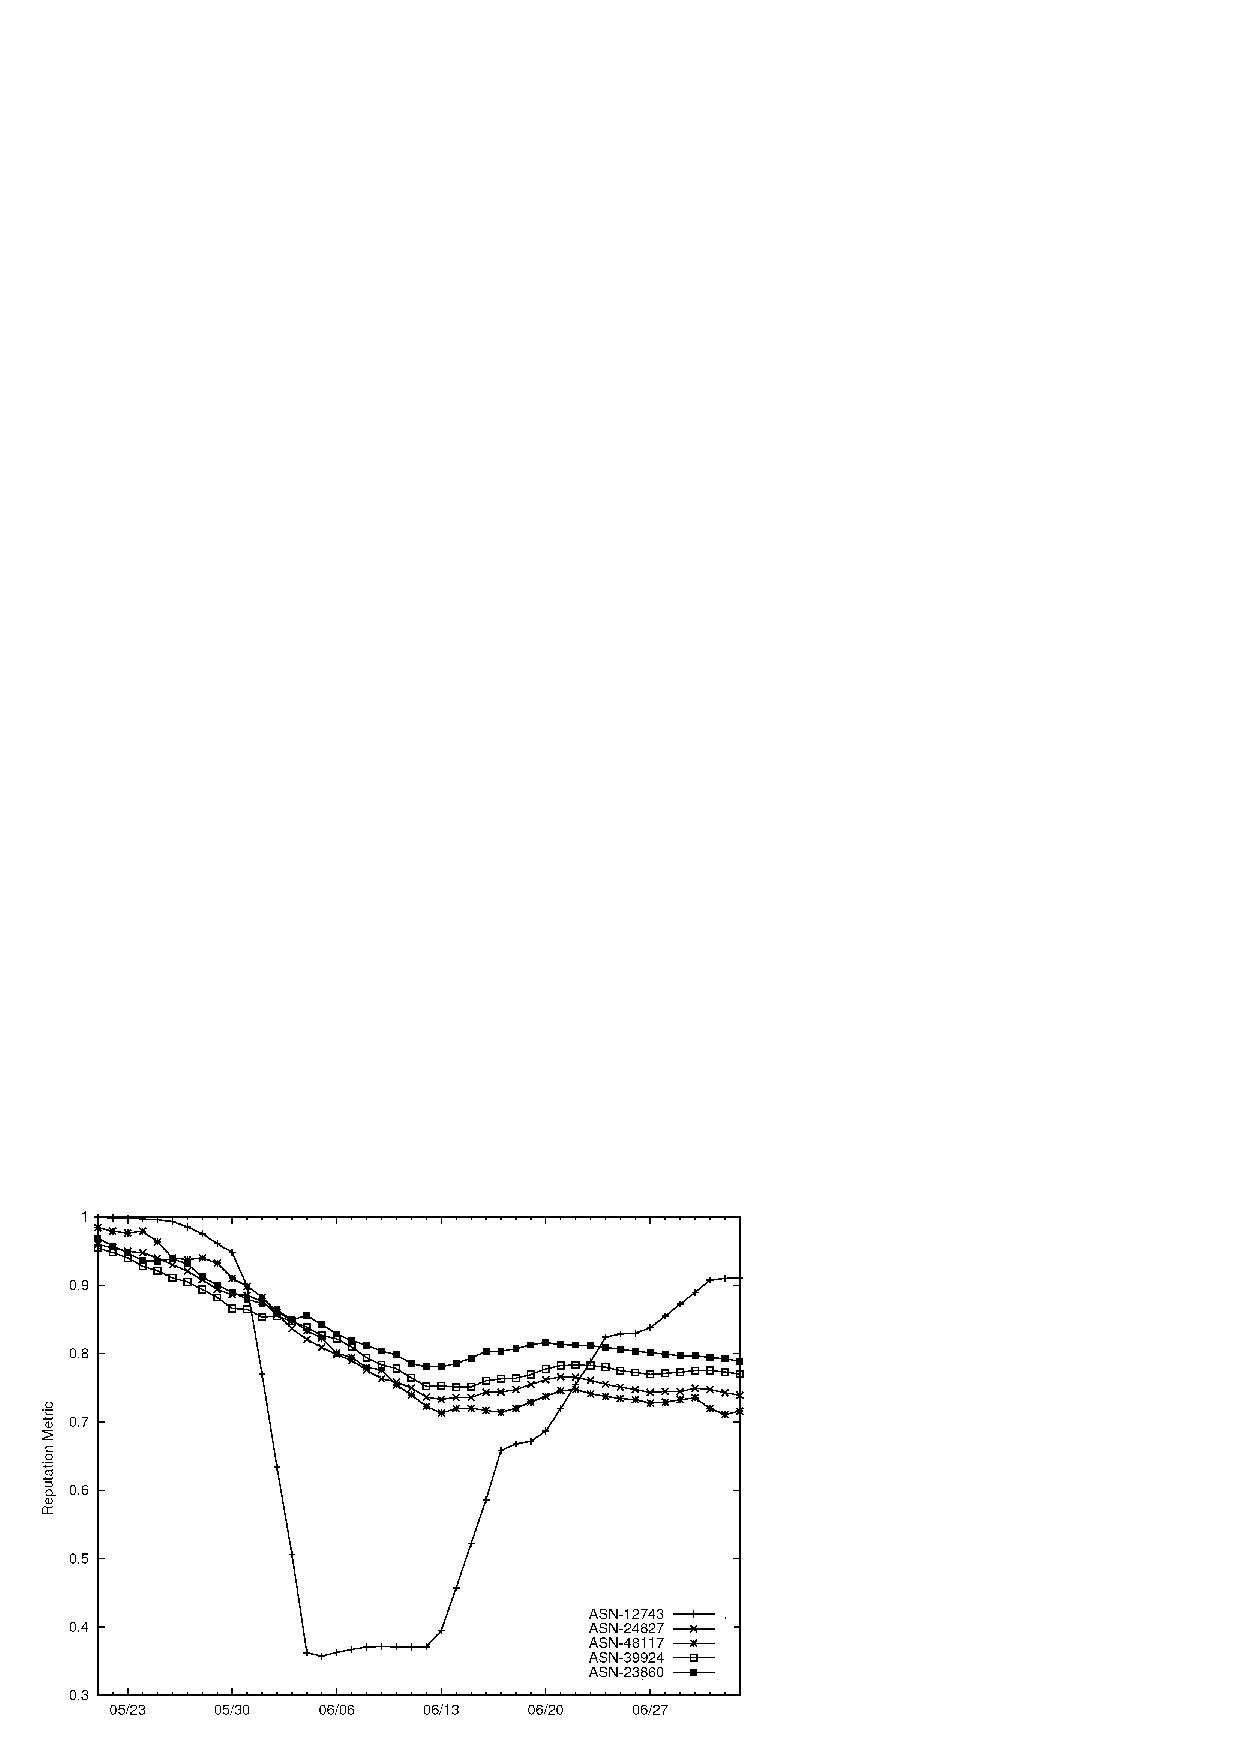
\includegraphics[width=0.75\linewidth]{some_graph}
	\end{center}
	\vspace{-12pt}
	\caption{Example Figure/Graph}
	\label{fig:some_graph}
\end{figure}

\end{document} 

